\section{Visualize Bragg Diffraction}

As individual runs or post-processed runs are completed, the output files will be placed in their respective directories specified in Table \ref{table_directory_struct}. The diffraction data is found in multiple directories: \fileio{GSAS}, \fileio{fullprof}, \fileio{topas}, and \fileio{rietveld}. Also, the \iptsPrint\fileio{/autoreduce} directory will have diffraction data as well. 

To visualize and plot the Bragg diffraction data, we use the \guicmd{Bragg Peaks} tab shown below and we view the files located in the \fileio{GSAS} directory: 

\noindent\makebox[\textwidth]{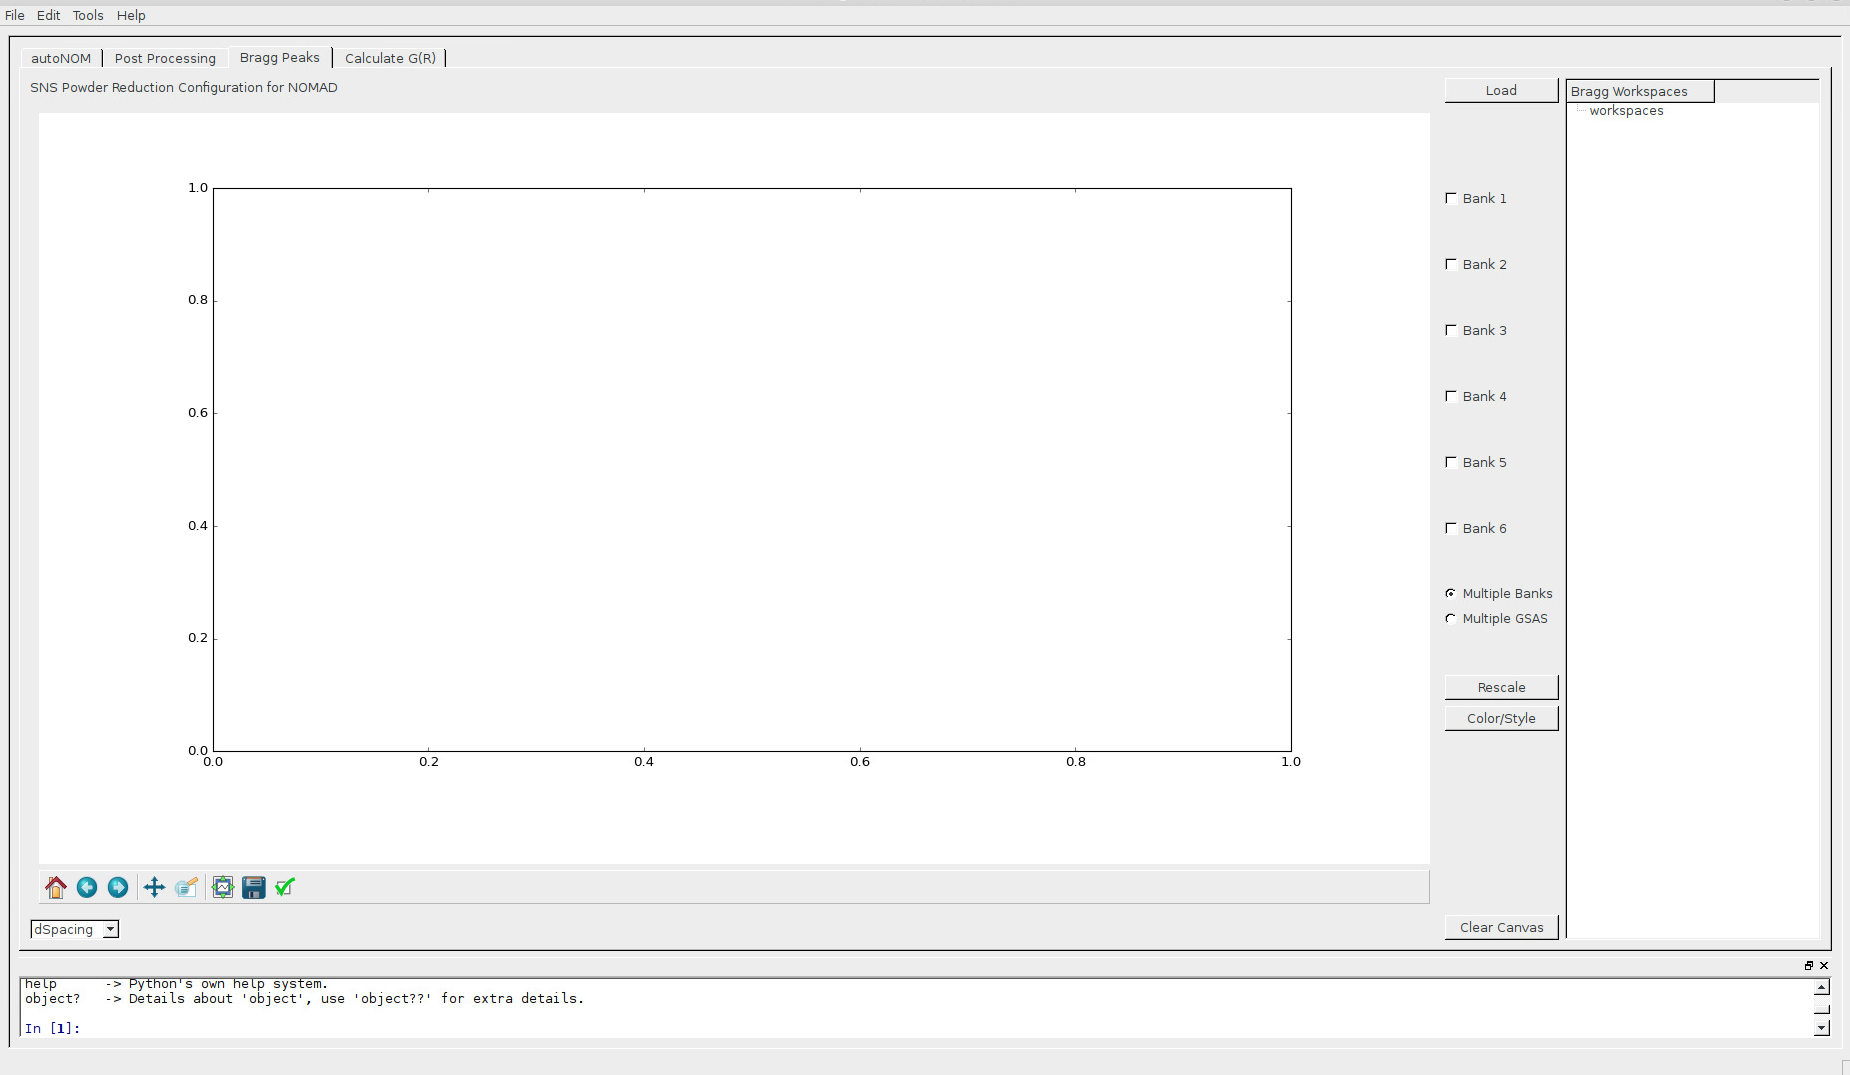
\includegraphics[width=0.9\paperwidth]{graphics/tab3/tab3.png}}

\subsection{Load Bragg data}

First we need to load in diffraction data. Go to the top right and press the \guicmd{Load} button. You should be presented with a file dialog similar to the one below:

\noindent\makebox[\textwidth]{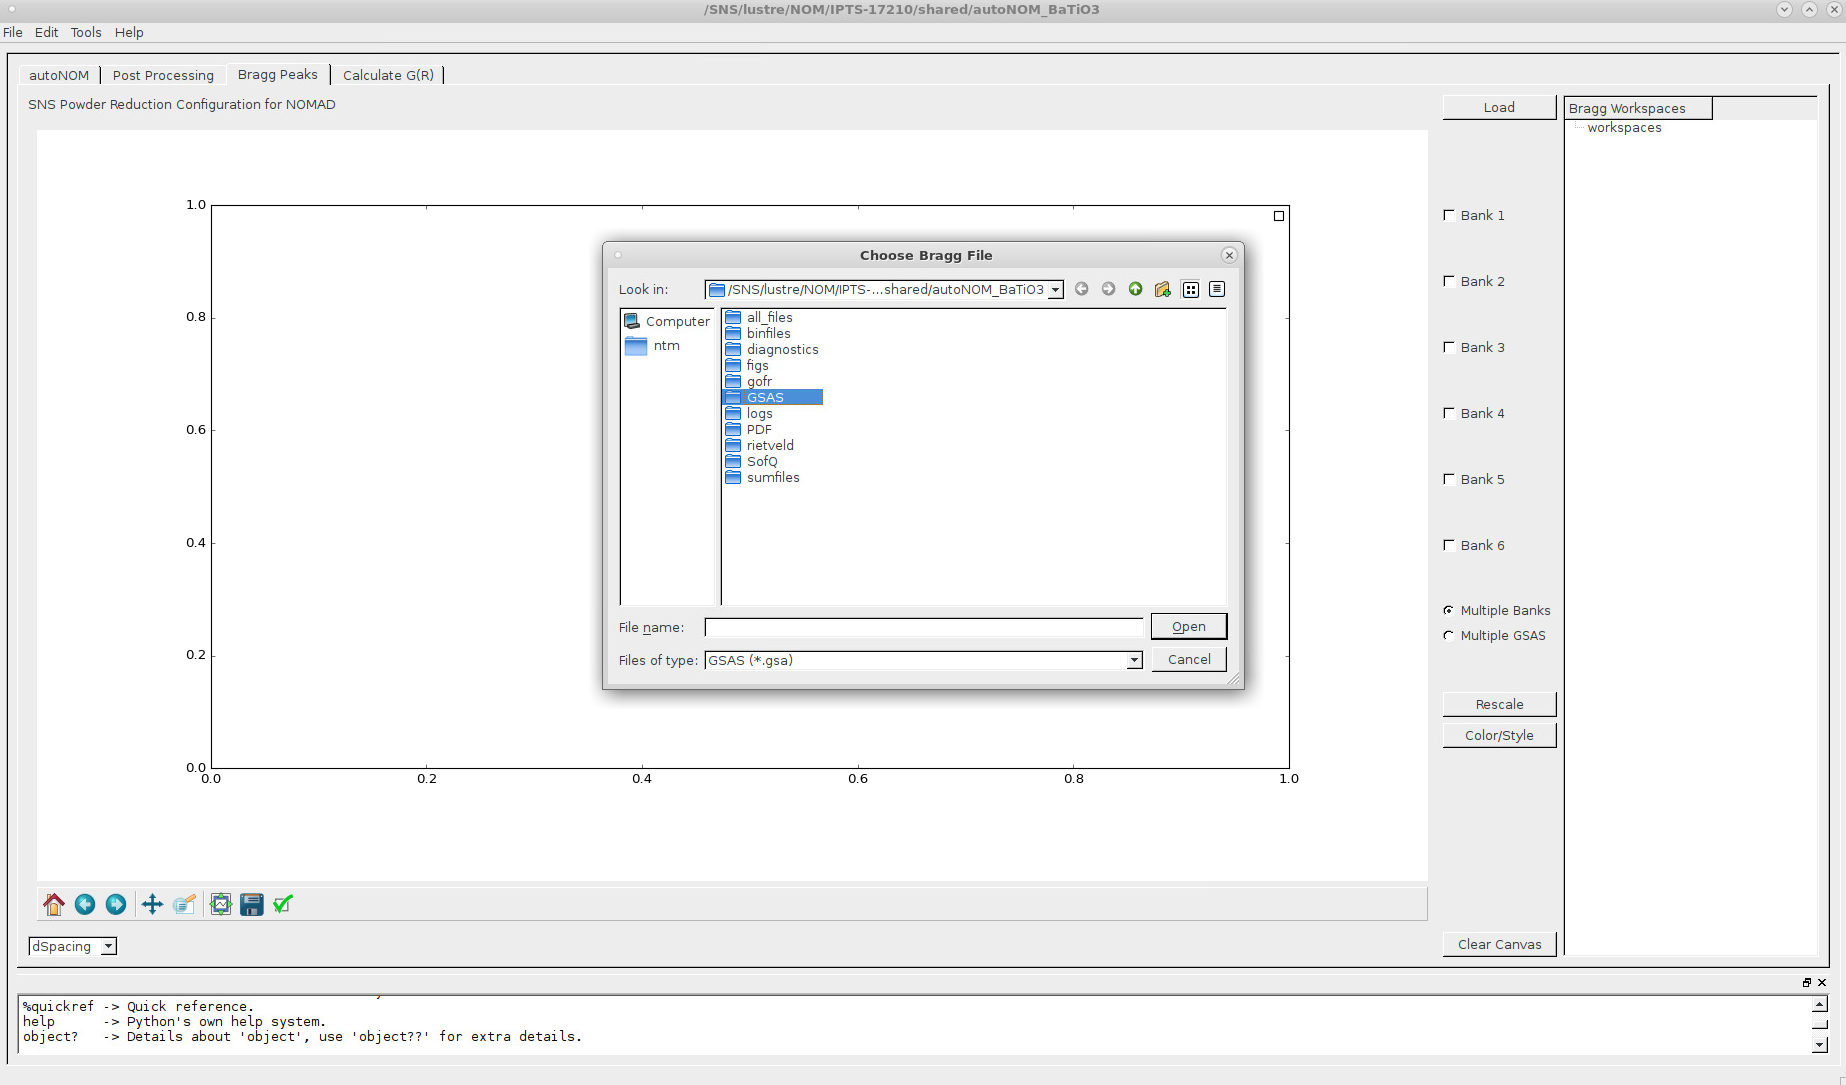
\includegraphics[width=0.9\paperwidth]{graphics/tab3/tab3_loadFiles.png}}

Double-click the \fileio{GSAS} diretory to see the files that are available. When you press \guicmd{Load}, you may actually start in the \fileio{GSAS} directory as well. From here, you can select individual runs, labeled as \fileio{NOM<run number>tof.gsa} or you can select post-processed runs such as summed files, labeled as \fileio{NOM\_<given title>.gsa}.  An example is displayed below:

\noindent\makebox[\textwidth]{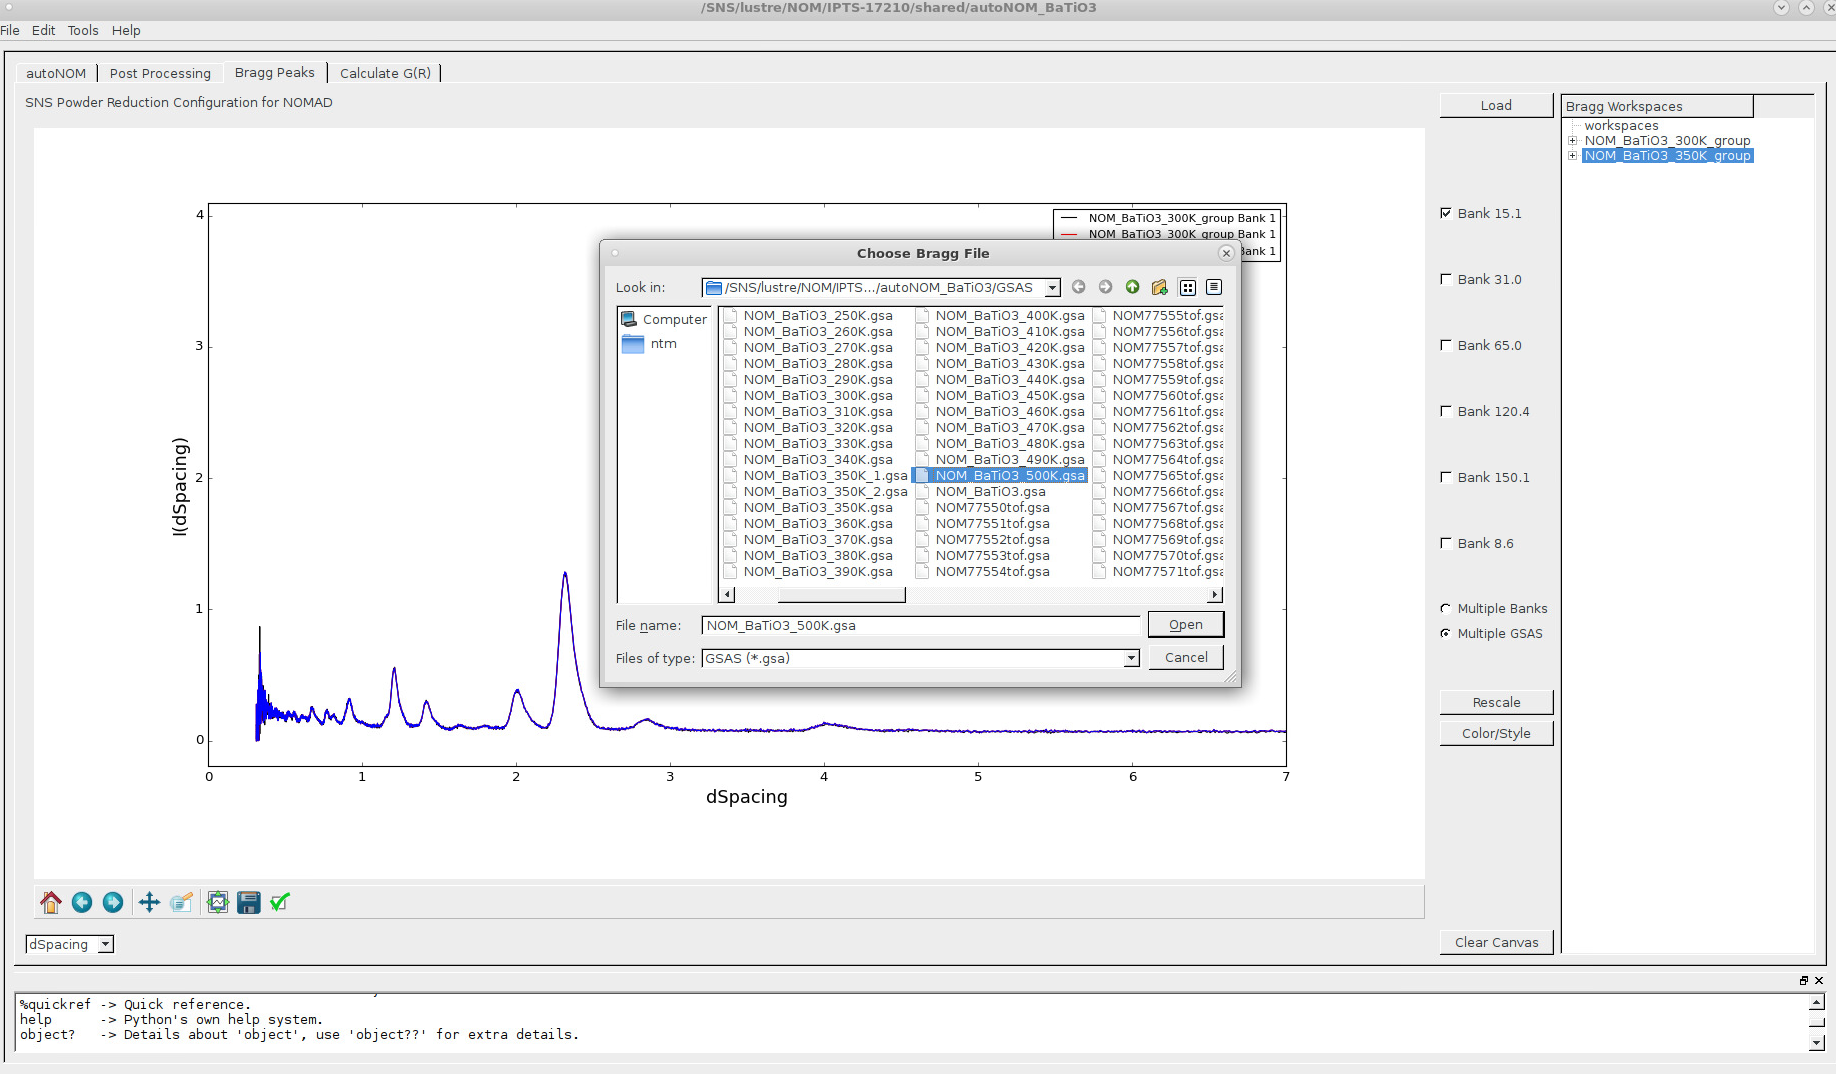
\includegraphics[width=0.9\paperwidth]{graphics/tab3/tab3_loadFiles_showIndiviuals.png}}

You can also select multiple individual runs while holding the \cmd{Ctrl} key or you can select a span of runs by holding the \cmd{Shift} key while selecting the runs. Once the runs are selected, press the \guicmd{Open} button. 

Below we show where we have loaded the summed run for 300K. 

\noindent\makebox[\textwidth]{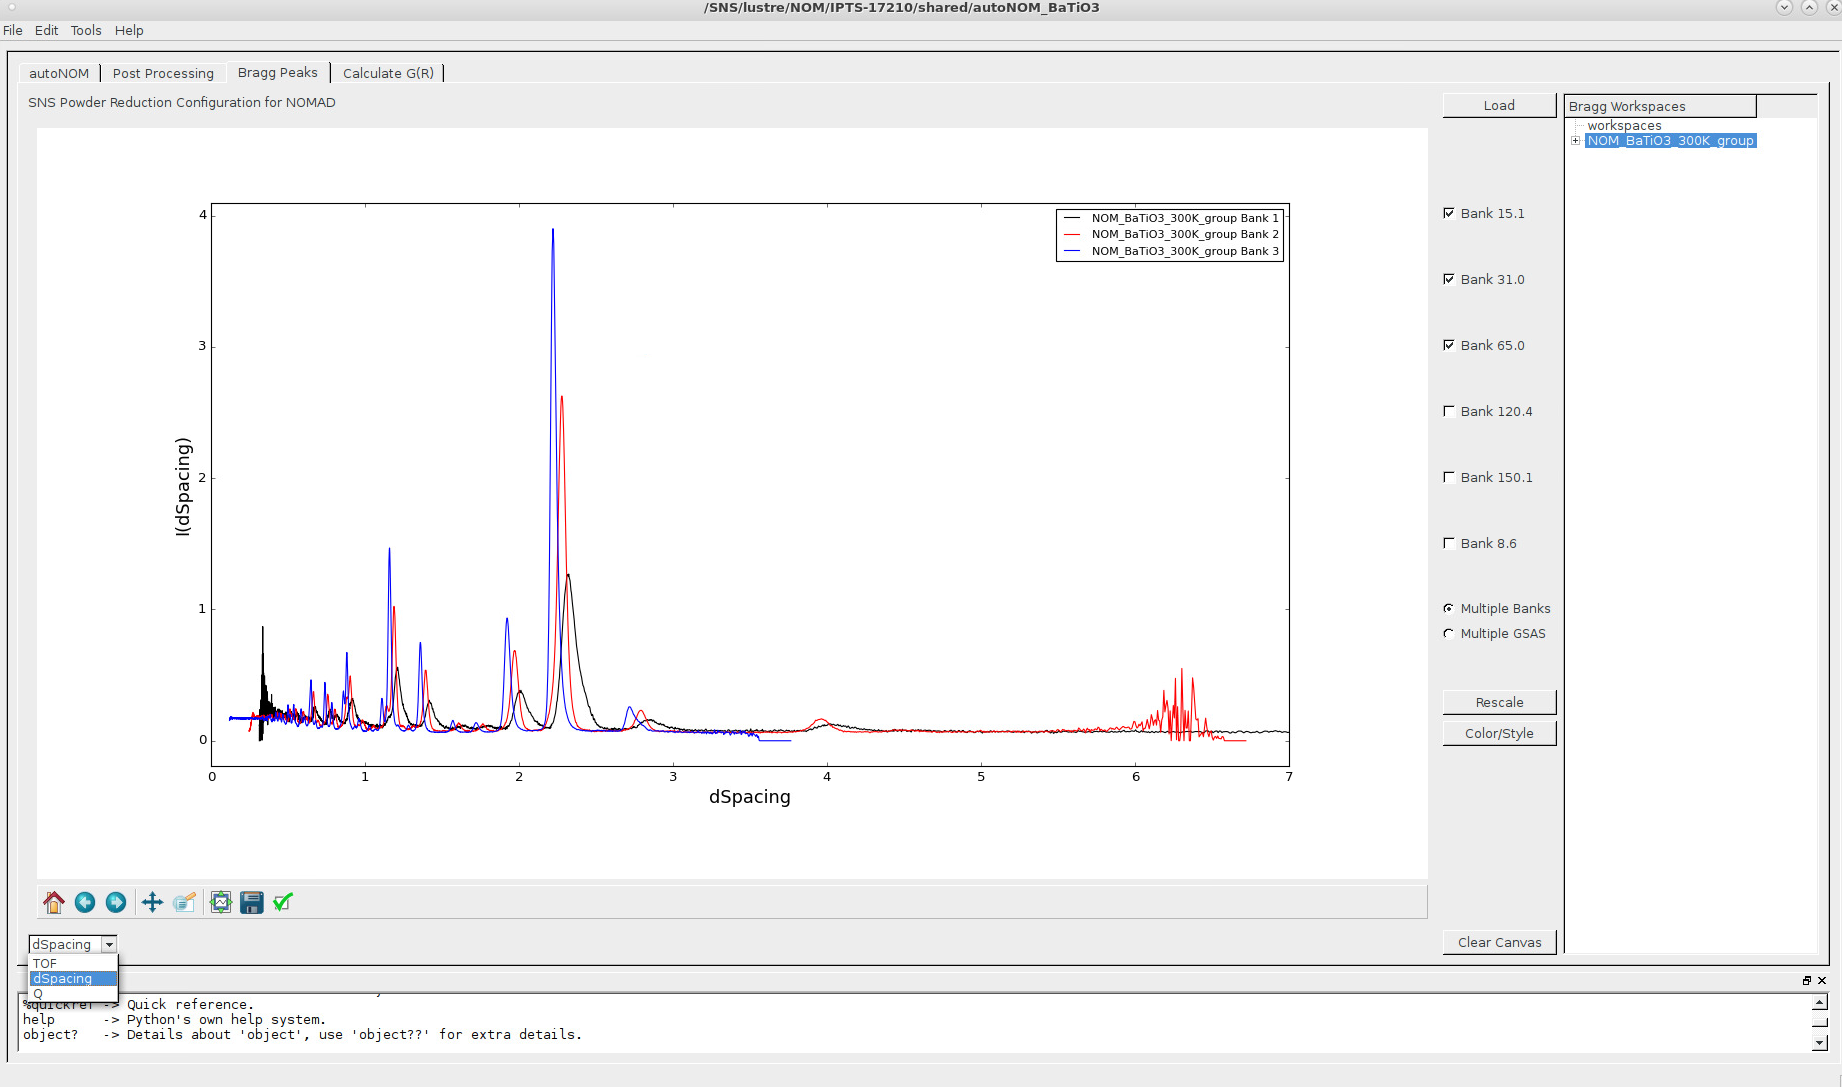
\includegraphics[width=0.9\paperwidth]{graphics/tab3/tab3_multipleBanks.png}} \label{fig_multiBraggBanks}

\subsection{Adjust Graphs}

This tab has two modes to view the diffraction data from the banks: \guicmd{Multiple Banks} and \guicmd{Multiple GSAS}. 

\begin{itemize}

\item \guicmd{Multiple Banks}: In this mode, we can view diffraction data from different banks of the same run. We can select the banks to display on the right-hand side. We can select multiple different banks in this mode.

\item \guicmd{Multiple GSAS}: In this mode, we can view diffraction data from different runs for a single bank. We can select the bank to display on the right-hand side. We can select only one bank at a time in this mode.

\end{itemize}

In Figure \ref{fig_multiBraggBanks}, we are in \guicmd{Multiple Banks} mode and have three of the banks selected. When we load in more than one dataset, we can use \guicmd{Multiple GSAS} mode. Below, we show where we have loaded in the 300K, 350K, and 500K data sets and have selected the 31.0 degree bank to view the data:

\noindent\makebox[\textwidth]{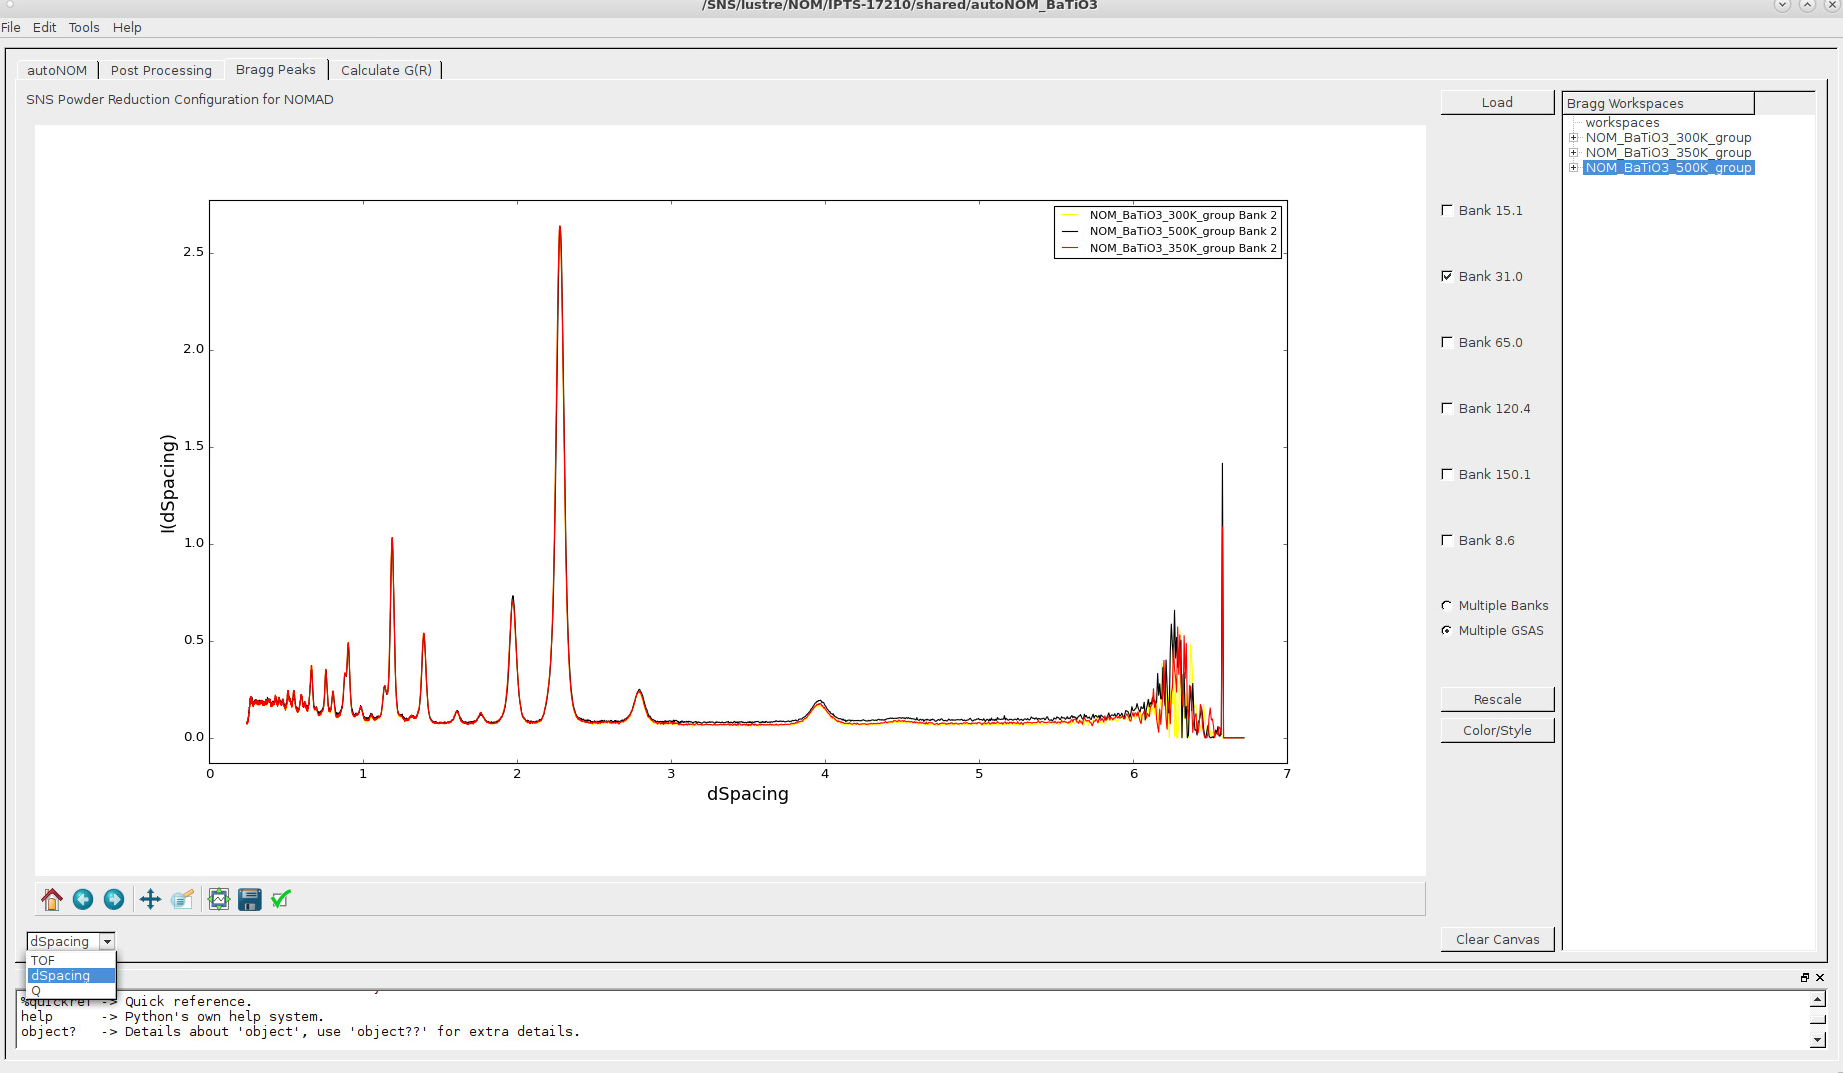
\includegraphics[width=0.9\paperwidth]{graphics/tab3/tab3_multipleGSAS.png}} \label{fig_multiBraggBanks}

Under the bank and mode selection, we have the \guicmd{Rescale} and \guicmd{Color/Style} buttons. The \guicmd{Rescale} button can be used to rescale the frame to better fit the data if the y-axis spans too far or not enought to capture the data. The \guicmd{Color/Style} button can be used to change the display of the data in the plot. After pressing the \guicmd{Color/Style} button, we are presented with a file dialog box. We can select the workspace from the drop-down list we would like to change, shown below, and can change the color of the curve, add markers, and select the fill and edge color of the markers from the other drop-downs: 

\noindent\makebox[\textwidth]{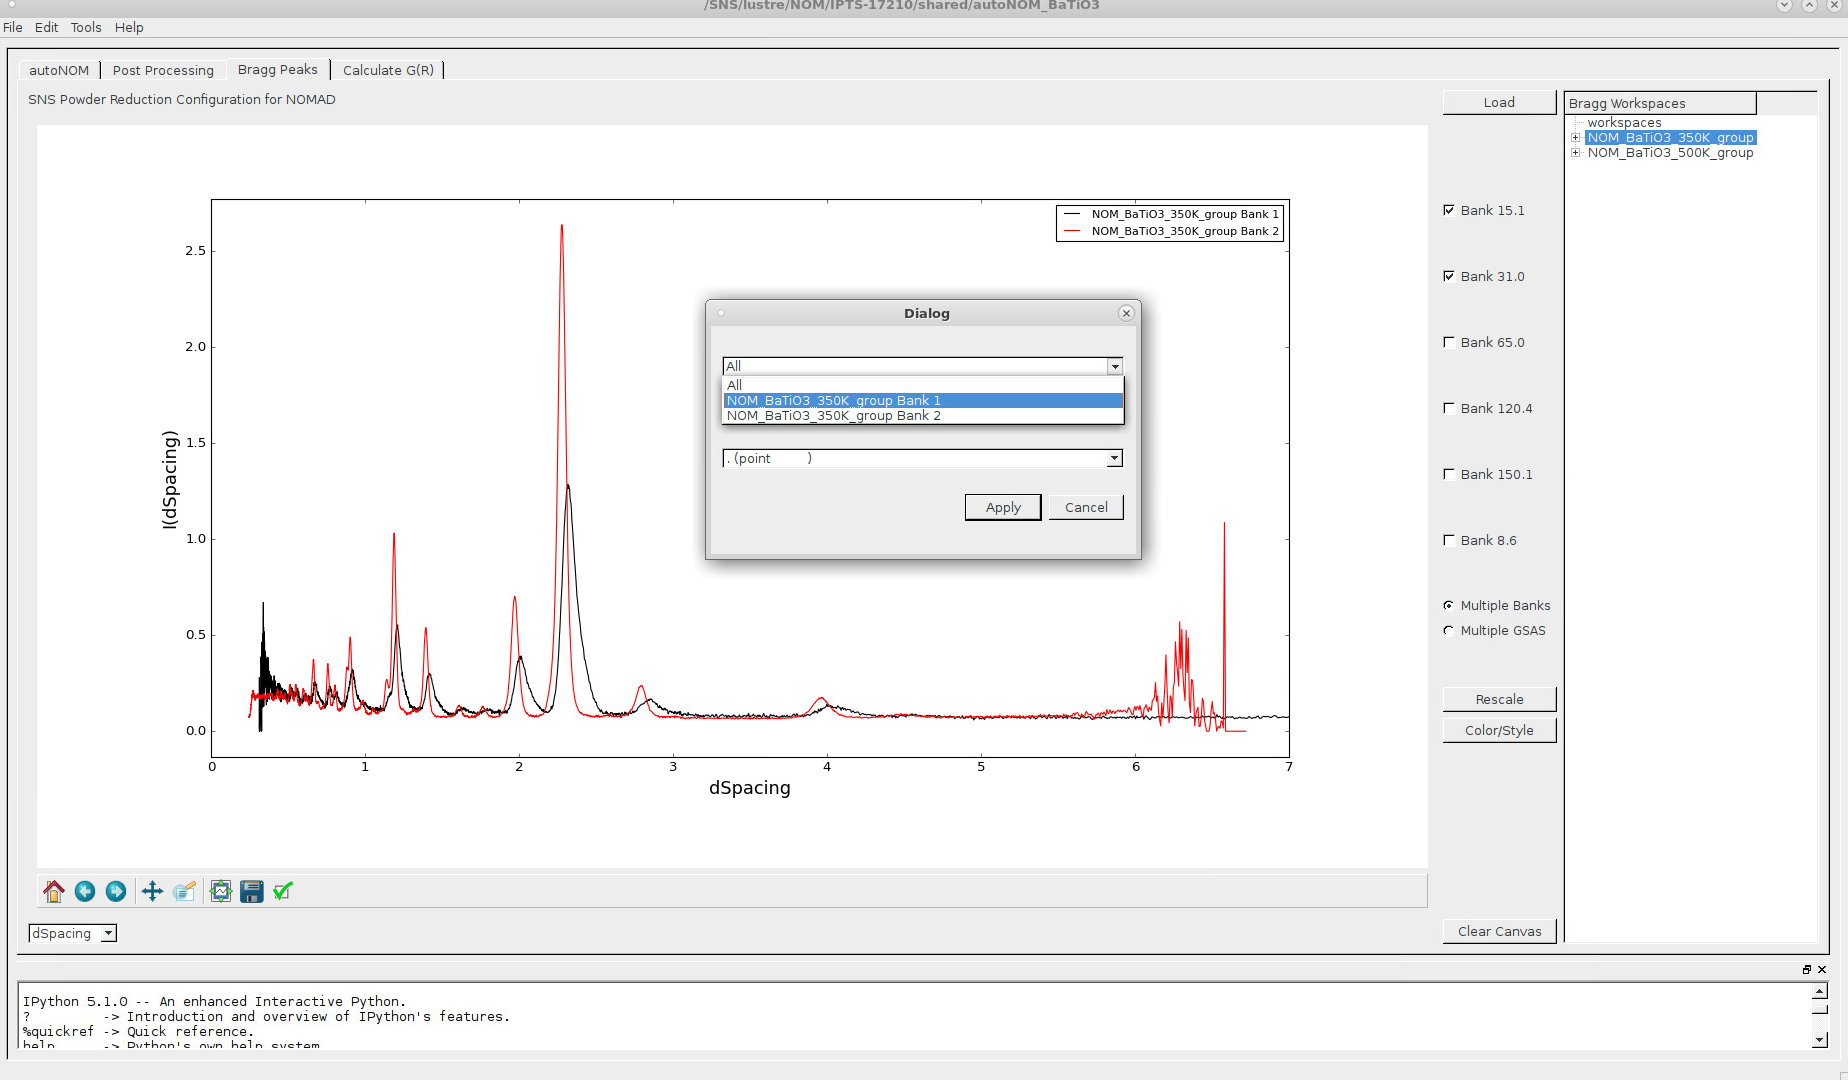
\includegraphics[width=0.9\paperwidth]{graphics/tab3/tab3_colorStyle.png}} 

Under the \guicmd{Rescale} and \guicmd{Color/Style}, we have the \guicmd{Clear Canvas} button. This can be used to quickly clear the plot of all datasets and begin again.

You will also notice in the bottom left of the tab space  that we can change the x-axis that we display the graph in. The choices are: \guicmd{TOF} for time-of-flight, \guicmd{dSpacing} for d-spacing (the default), and \guicmd{Q} for momentum transfer. The graph will change accordingly. 

For each of the datasets that have been loaded, we have a \guicmd{Bragg Workspaces} tree on the far right side. If you right-click on any of the workspaces, you will see the following options, demonstrated below:

\noindent\makebox[\textwidth]{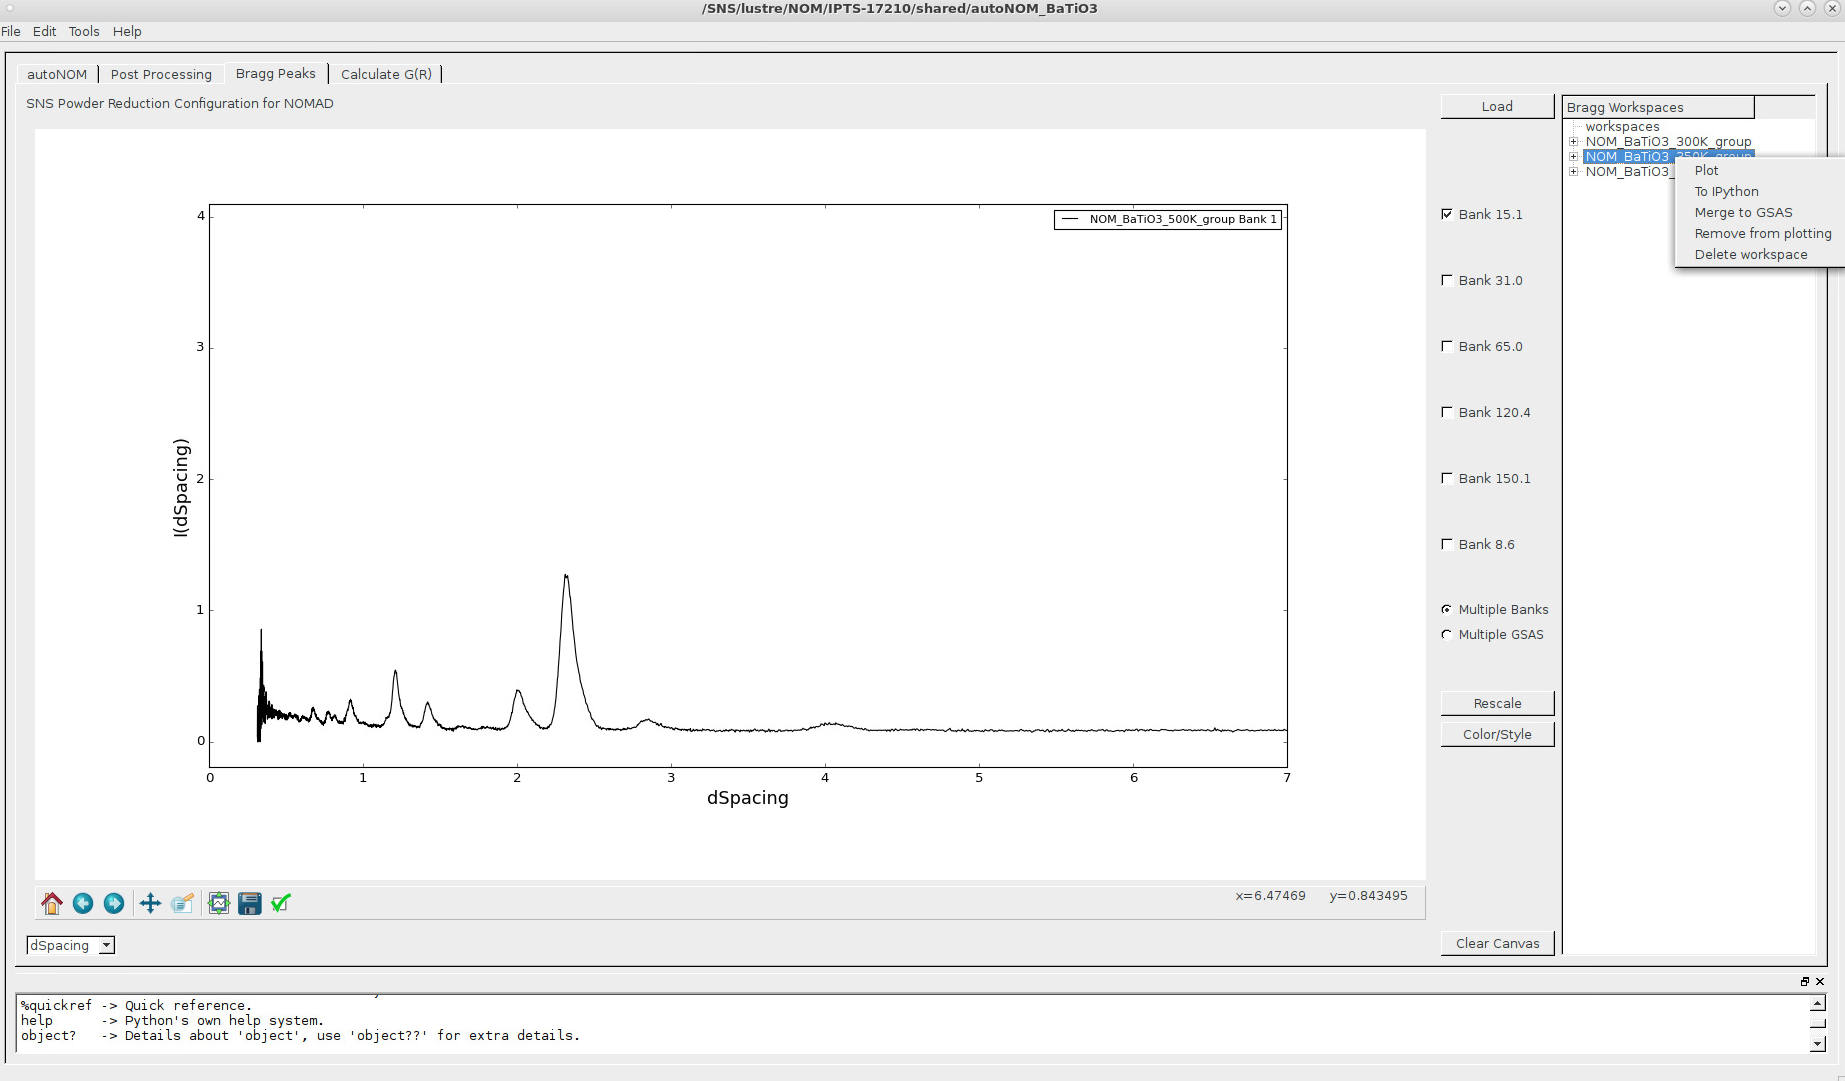
\includegraphics[width=0.9\paperwidth]{graphics/tab3/tab3_rightClick.png}} 

From the options, you can do the following:

\begin{itemize}

\item \guicmd{Plot}: Plot the selected workspace on the graph area.

\item \guicmd{To IPython}: Transfer the workspace to the IPython command line dock at the bottom. Here, you can script changes to the workspace and output a new workspace. If clicked, you will have something similar to what is shown below:

\noindent\makebox[\textwidth]{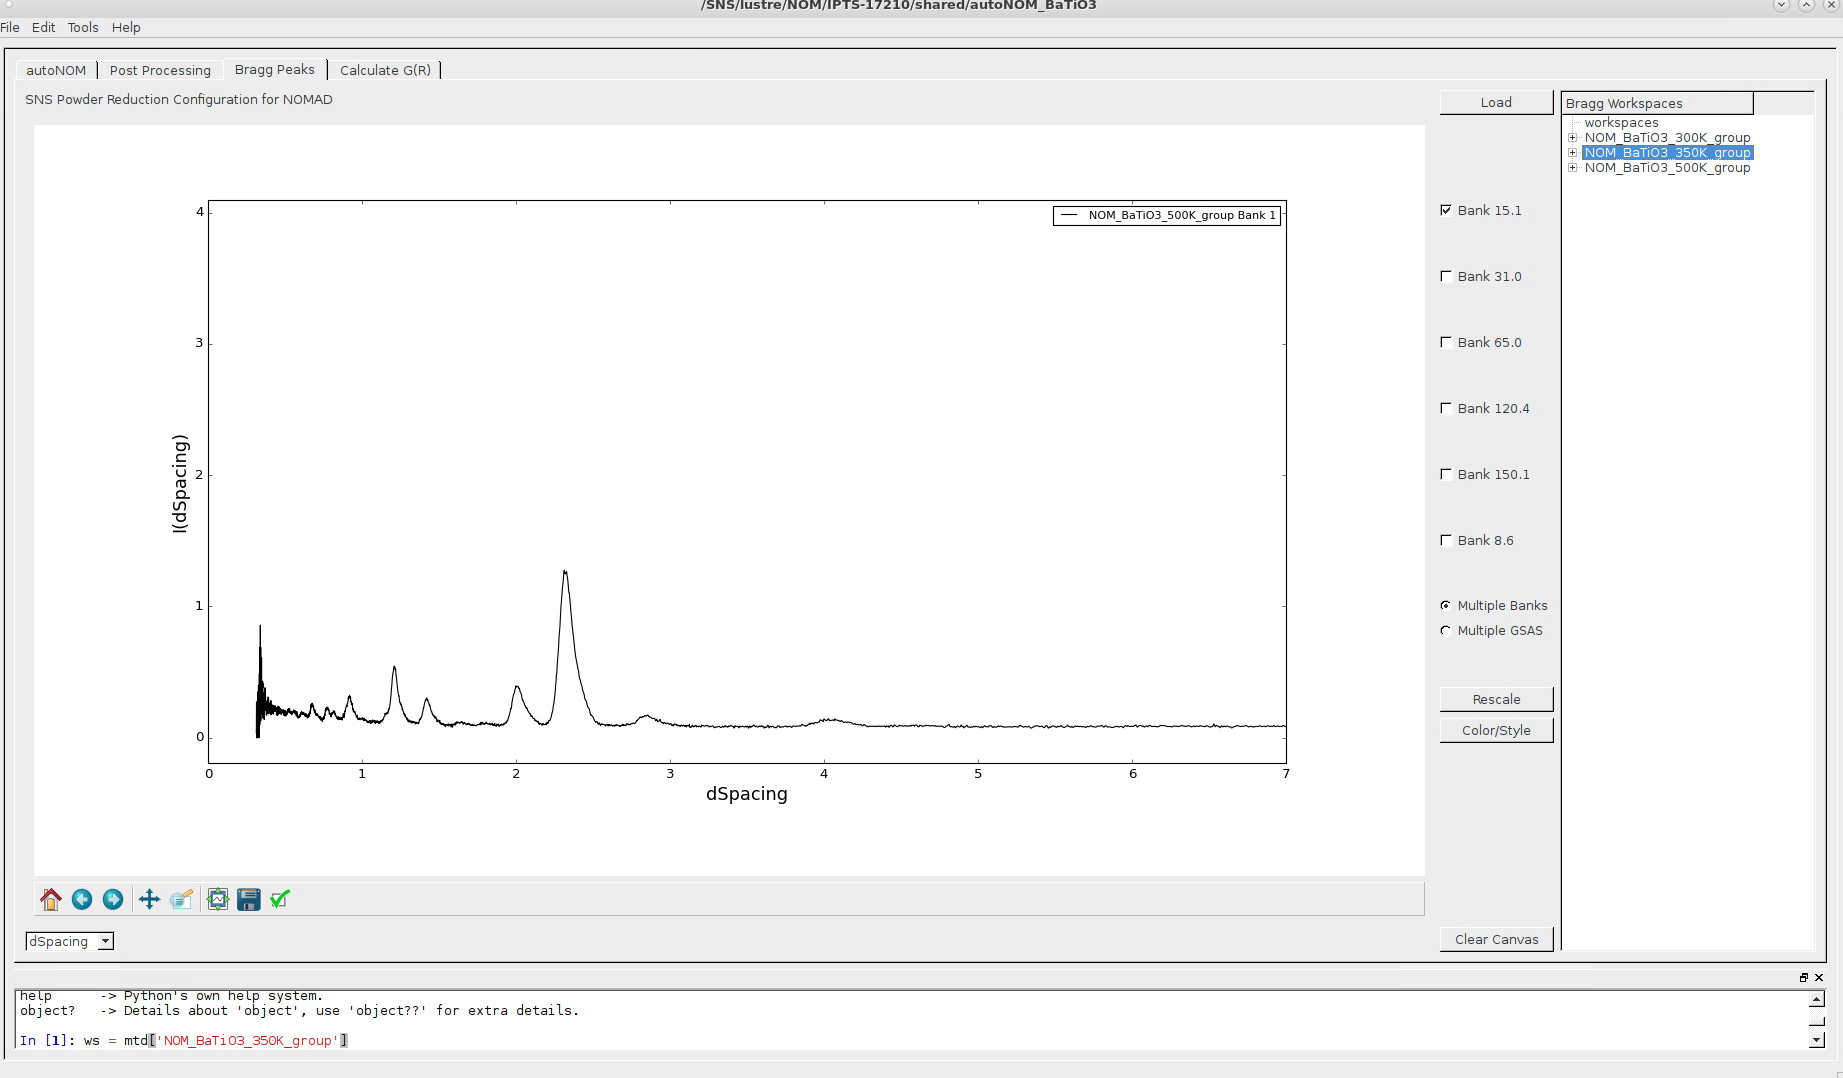
\includegraphics[width=0.8\paperwidth]{graphics/tab3/tab3_rightClick_toIPython.png}}

You can "undock" the IPython command line dock by pressing the double-window icon in the top right of the dock, shown below:

\noindent\makebox[\textwidth]{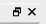
\includegraphics[width=0.1\paperwidth]{graphics/tab3/tab3_rightClick_icon.png}} 

This will allow you to expand and contract the IPython command line dock. At anytime, you can redock by pressing the same double-window icon in the top right of the dock:

\noindent\makebox[\textwidth]{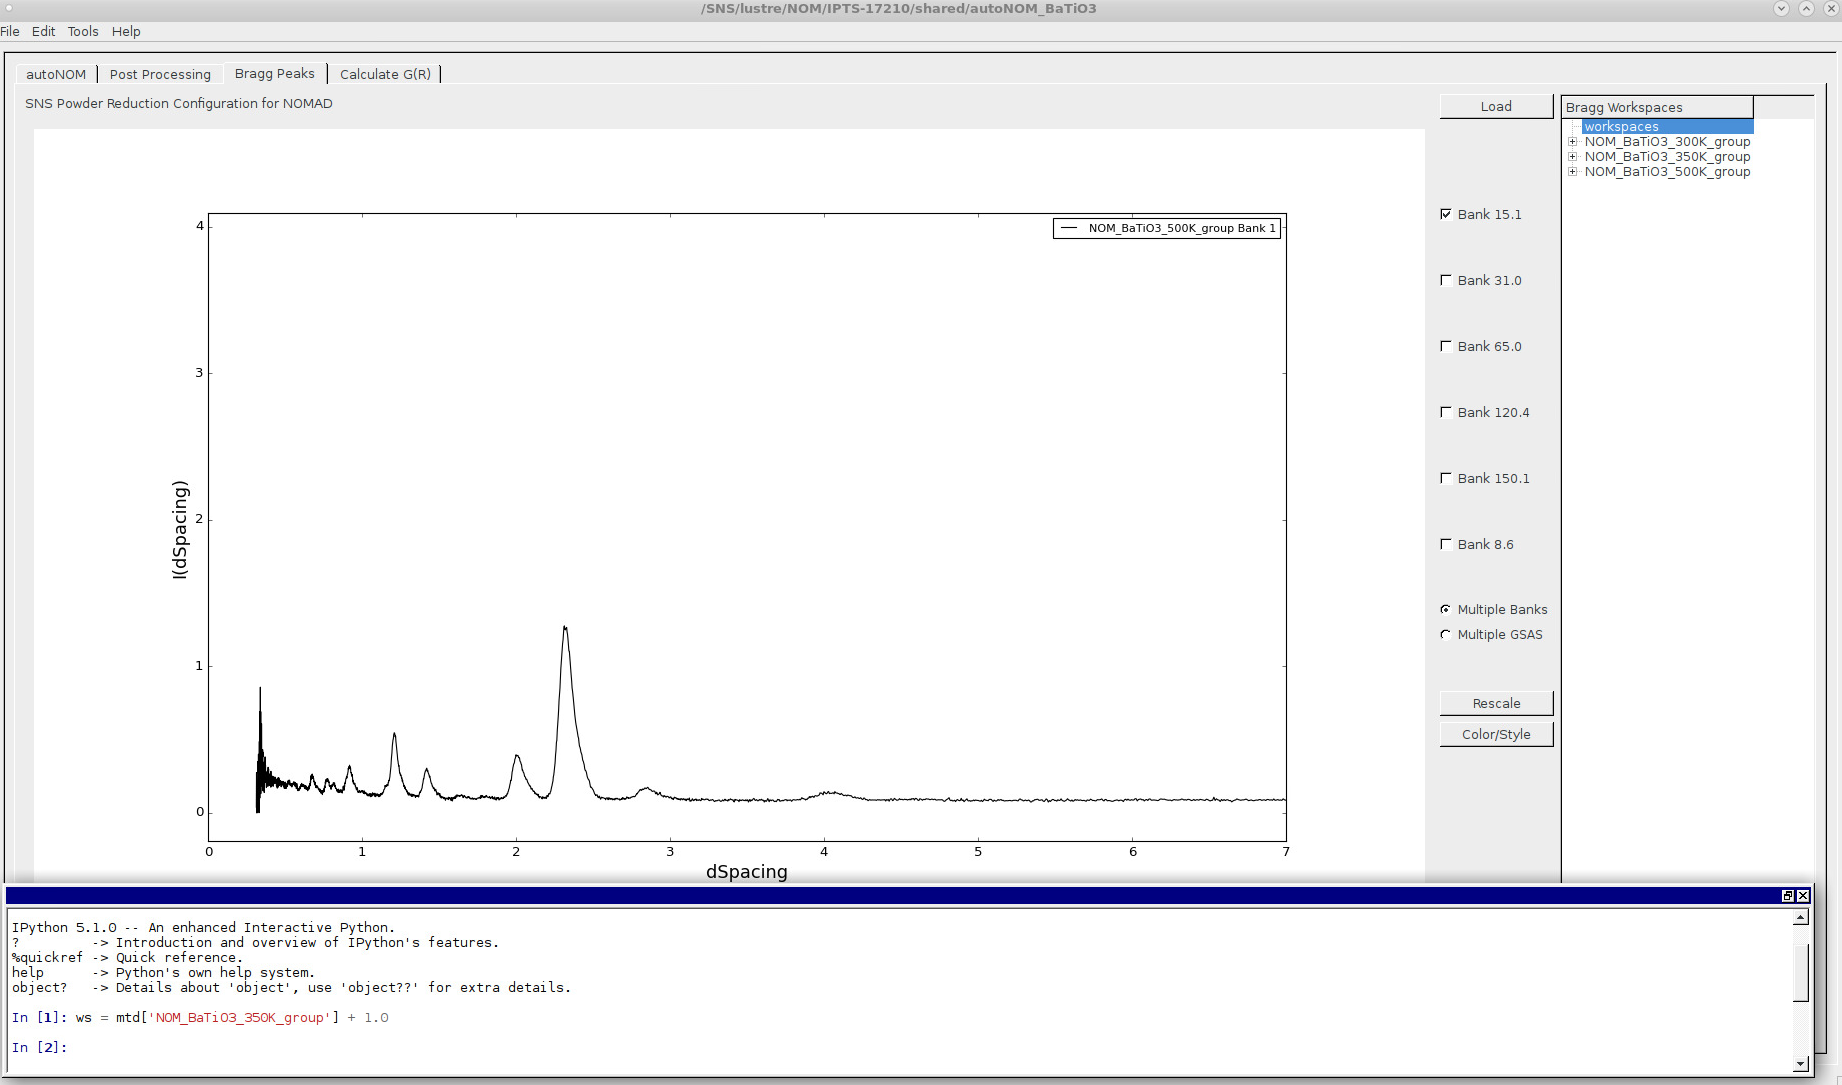
\includegraphics[width=0.8\paperwidth]{graphics/tab3/tab3_rightClick_toIPython_unDock.png}}

\item \guicmd{Merge to GSAS}: Will give a merged GSAS output file of the banks.
\item \guicmd{Remove from plotting}: Removes dataset from the plot.
\item \guicmd{Delete workspace}: Deletes the dataset from the \guicmd{Bragg Workspaces} tree.

\end{itemize}

To change the legend, in case it is in the way or masking data, you can right-click inside any of the plot areas and either reduce the font of the text, increase the font of the text, or hide the legend all together.



